\documentclass[12pt,a4paper,oneside]{report}             % Single-side


\usepackage{ifxetex}
\ifxetex
  \usepackage{fontspec}
\else
  \usepackage[T1]{fontenc}
  \usepackage[utf8]{inputenc}
  \usepackage{lmodern}
\fi

\usepackage[magyar]{babel} % Alapértelmezés szerint utoljára definiált nyelv lesz aktív, de később külön beállítjuk az aktív nyelvet.

\usepackage{combelow}
\usepackage{newunicodechar}

\newunicodechar{Ș}{\cb{S}}
\newunicodechar{ș}{\cb{s}}
\newunicodechar{Ț}{\cb{T}}
\newunicodechar{ț}{\cb{t}}

\usepackage{cmap}
\usepackage{amsfonts,amsmath,amssymb} % Mathematical symbols.
\usepackage[ruled,boxed,resetcount,linesnumbered]{algorithm2e} % For pseudocodes.
\def\algorithmcfname{algoritmus}
\makeatletter
\renewcommand{\fnum@algocf}{\AlCapSty{\AlCapFnt\thealgocf.\nobreakspace\algorithmcfname}}
\makeatother

\usepackage{booktabs} % For publication quality tables for LaTeX
\usepackage{graphicx}
\usepackage{sidecap}

%\usepackage{fancyhdr}
%\usepackage{lastpage}

\usepackage{anysize}
\usepackage{sectsty}
\usepackage{setspace}  % Ettol a tablazatok, abrak, labjegyzetek maradnak 1-es sorkozzel!

% For hyperlinks in the generated document. 
\usepackage{color}
\usepackage{listings} % For source code snippets.

%\usepackage[amsmath,thmmarks]{ntheorem} % Theorem-like environments.

\usepackage[hang]{caption}
\usepackage{scrextend}

\usepackage{indentfirst}
\usepackage{pdfpages}

\usepackage{xfrac}
\usepackage{eurosym}

\usepackage{fullpage} % a margokra is lehessen irni

\newcommand{\vigyazat}{\marginpar{\textcolor{red}{\emph{Vigy\'azat!}}}}

\usepackage{tikz}
\usepackage{verbatim}
\usetikzlibrary{arrows,shapes}
\usetikzlibrary{positioning}
\tikzset{main node/.style={circle,fill=blue!20,draw,minimum size=1cm,inner sep=0pt},
}
\onehalfspacing % Add this command to set the line spacing to 1.5
%--------------------------------------------------------------------------------------
% Language configuration -- choose one
%--------------------------------------------------------------------------------------
%--------------------------------------------------------------------------------------
% Elnevezések
%--------------------------------------------------------------------------------------
\newcommand{\dolgozatnyelve}{\selectlanguage{magyar}}



\newcommand{\bsc}{Diplomadolgozat}
\newcommand{\msc}{Disszert\'aci\'os dolgozat}

\newcommand{\pelda}{Példa}
\newcommand{\definicio}{Definíció}
\newcommand{\tetel}{Tétel}

\newcommand{\bevezeto}{Bevezető}
\newcommand{\koszonetnyilvanitas}{Köszönetnyilvánítás}
\newcommand{\abrakjegyzeke}{Ábrák jegyzéke}
\newcommand{\tablazatokjegyzeke}{Táblázatok jegyzéke}
\newcommand{\irodalomjegyzek}{Irodalomjegyzék}
\newcommand{\fuggelek}{Függelék}


\newcommand{\englishParagraph}{
	\setlength{\parindent}{0em} % angol nyelvű dokumentumokban jellemző
	\setlength{\parskip}{0.5em} % angol nyelvű dokumentumokban jellemző
	\nonfrenchspacing
}

\newcommand{\hungarianParagraph}{
	\setlength{\parindent}{2em} % angol nyelvű dokumentumokban jellemző
	\setlength{\parskip}{0em}   % angol nyelvű dokumentumokban jellemző
	\frenchspacing
}

\newcommand{\defaultParagraph}{
	\hungarianParagraph
}  % Beállítások magyar nyelvű dolgozathoz

%--------------------------------------------------------------------------------------
% Main variables
%--------------------------------------------------------------------------------------



% Szak alapkepzes
\newcommand{\szakHU}{INFORMATIKA SZAK}
\newcommand{\szakRO}{SPECIALIZAREA INFORMATIC\v A}
\newcommand{\szakEN}{COMPUTER SCIENCE SPECIALIZATION}


\newcommand{\dolgozattipusHU}{DIPLOMADOLGOZAT}
\newcommand{\dolgozattipusRO}{LUCRARE DE DIPLOM\v A}
\newcommand{\dolgozattipusEN}{BACHELOR THESIS}

\newcommand{\szerzo}{Füzi Zalán} % Szerző neve
\newcommand{\temavezetoA}{Dr. Márton Gyöngyvér} % Vezetőtanár neve


% Fokozatok

%Egyetemi tan\'ar/ Profesor universitar/Full Professor
%Egyetemi docens/ Conferențiar universitar/Associate professor
%Egyetemi adjunktus/Lector universitar sau Șef de lucrări /Lecturer
%Egyetemi tan\'arseg\'ed/Asistent universitar/Assistant professor


\newcommand{\temavezetoAfokozat}{Egyetemi adjunktus}% Első konzulens neve
\newcommand{\temavezetoAfokozatRo}{Lector universitar}
\newcommand{\temavezetoAfokozatEn}{Lecturer}
\newcommand{\temavezetoB}{} % Második konzulens neve
\newcommand{\cimHu}{Cryptorithm} % Cím
\newcommand{\cimRO}{Cryptorithm}
\newcommand{\cimEN}{Cryptorithm}
\newcommand{\ev}{2023} %az aktualis ev

%--------------------------------------------------------------------------------------
% Page layout setup
%--------------------------------------------------------------------------------------
% we need to redefine the pagestyle plain
% another possibility is to use the body of this command without \fancypagestyle
% and use \pagestyle{fancy} but in that case the special pages
% (like the ToC, the References, and the Chapter pages)remain in plane style

\usepackage{smartdiagram}
\usepackage{tikz,pgf}
\usepackage{pgfplots}
\pgfplotsset{width=7cm,compat=1.8}
\usetikzlibrary{matrix,calc,shapes}

\tikzset{
	treenode/.style = {shape=rectangle, rounded corners, draw, anchor=center, text width=5em, align=center, top color=white, bottom color=blue!20,inner sep=1ex},
	decision/.style = {treenode, diamond, inner sep=0pt},
	root/.style = {treenode, font=\Large, bottom color=red!30},
	env/.style = {treenode, font=\ttfamily\normalsize},
	finish/.style = {root, bottom color=green!40},
	dummy/.style = {circle,draw}
}


\setcounter{secnumdepth}{0}
\sectionfont{\large\upshape\bfseries}
\setcounter{secnumdepth}{2}

\sloppy % Margón túllógó sorok tiltása.
\widowpenalty=10000 \clubpenalty=10000 %A fattyú- és árvasorok elkerülése
\def\hyph{-\penalty0\hskip0pt\relax} % Kötőjeles szavak elválasztásának engedélyezése


%--------------------------------------------------------------------------------------
% Setup hyperref package
%--------------------------------------------------------------------------------------
\usepackage{xcolor}
\definecolor{bluecite}{HTML}{0875b7}
\usepackage[unicode=true,
bookmarksopen={true},
pdffitwindow=true, 
colorlinks=true, 
linkcolor=bluecite, 
citecolor=bluecite, 
urlcolor=bluecite, 
hyperfootnotes=false, 
pdfstartview={FitH},
pdfpagemode= UseNone]{hyperref}


%--------------------------------------------------------------------------------------
% Set up listings
%--------------------------------------------------------------------------------------



\definecolor{codegreen}{rgb}{0,0.6,0}
\definecolor{codegray}{rgb}{0.5,0.5,0.5}
\definecolor{codepurple}{rgb}{0.58,0,0.82}
\definecolor{backcolour}{rgb}{0.95,0.95,0.92}




\definecolor{lightgray}{rgb}{0.95,0.95,0.95}
\definecolor{darkgreen}{RGB}{3,125,80}
\lstset{frame=tb,
	language=Matlab,
	aboveskip=3mm,
	belowskip=3mm,
	showstringspaces=false,
	columns=flexible,
	basicstyle={\small\ttfamily},
	numbers=none,
	numberstyle=\tiny\color{gray},
	keywordstyle=\color{blue},
	commentstyle=\color{codegreen},
	%stringstyle=\color{mauve},
	breaklines=true,
	breakatwhitespace=true,
	tabsize=3,
	backgroundcolor=\color{lightgray},
}
\def\lstlistingname{k\'odr\'eszlet}	


%--------------------------------------------------------------------------------------
% Set up theorem-like environments
%--------------------------------------------------------------------------------------
% Using ntheorem package -- see http://www.math.washington.edu/tex-archive/macros/latex/contrib/ntheorem/ntheorem.pdf
%\swapnumbers
%\theoremstyle{plain}
%\theoremseparator{.}
\newtheorem{example}{\pelda}[section]

%\theoremseparator{.}
%\theoremprework{\bigskip\hrule\medskip}
%\theorempostwork{\hrule\bigskip}
%\theorembodyfont{\upshape}
%\theoremsymbol{{\large \ensuremath{\centerdot}}}
\newtheorem{definition}{\definicio}[section]

%\theoremseparator{.}
%\theoremprework{\bigskip\hrule\medskip}
%\theorempostwork{\hrule\bigskip}
\newtheorem{theorem}{\tetel}[section]

\newtheorem{conclusion}{Következtetés}[section]


%--------------------------------------------------------------------------------------
% Some new commands and declarations
%--------------------------------------------------------------------------------------
\newcommand{\code}[1]{{\upshape\ttfamily\scriptsize\indent #1}}
\newcommand{\doi}[1]{DOI: \href{http://dx.doi.org/\detokenize{#1}}{\raggedright{\texttt{\detokenize{#1}}}}} % A hivatkozások közt így könnyebb DOI-t megadni.

\DeclareMathOperator*{\argmax}{arg\,max}
%\DeclareMathOperator*[1]{\floor}{arg\,max}
\DeclareMathOperator{\sign}{sgn}
\DeclareMathOperator{\rot}{rot}


%--------------------------------------------------------------------------------------
% Setup captions
%--------------------------------------------------------------------------------------

\captionsetup[figure]{
	width=.75\textwidth,
	aboveskip=10pt}
\renewcommand{\captionlabelfont}{\bf}
%\renewcommand{\captionfont}{\footnotesize\it}


%--------------------------------------------------------------------------------------
% Redefine reference style
%--------------------------------------------------------------------------------------
\newcommand{\figref}[1]{\ref{fig:#1}.}
\renewcommand{\eqref}[1]{(\ref{eq:#1})}
\newcommand{\listref}[1]{\ref{listing:#1}.}
\newcommand{\sectref}[1]{\ref{sect:#1}}
\newcommand{\tabref}[1]{\ref{tab:#1}.}





%--------------------------------------------------------------------------------------
% Table of contents and the main text
%--------------------------------------------------------------------------------------
\begin{document}
	
% CIMOLDALAK
%~~~~~~~~~~~~~~~~~~~~~~~~~~~~~~~~~~~~~~~~~~~~~~~~~~~~~~~~~~~~~~~~~~~~~~~~~~~~~~~~~~~~~~
	%--------------------------------------------------------------------------------------
%	A magyar cimoldal
%--------------------------------------------------------------------------------------
\begin{titlepage}
	\begin{center}
	
		\large{\bfseries SAPIENTIA ERDÉLYI MAGYAR TUDOMÁNYEGYETEM} \\
		\large{\bfseries MAROSVÁSÁRHELYI KAR,} \\
		\large{\bfseries \szakHU} \\[2.5cm]
			\begin{center}
			
\includegraphics[scale=2]{images/sapientia-hu}
		\end{center}
		\vspace{0.4cm}
		\Large{\Large  \cimHu}\\[0.8cm]
		\vspace{0.2cm}
		\textsc{\Large \bfseries \dolgozattipusHU}\\[2.5cm]
		
		{
			\large
		
			\renewcommand{\arraystretch}{0.85}
			\begin{tabular}{cc}
				 \makebox[6.5cm]{Témavezető:} & \makebox[6.5cm]{Végzős hallgató:} \\ \noalign{\smallskip}
				 \makebox[6.5cm]{\temavezetoA,} & \makebox[6.5cm]{\szerzo} \\ {\temavezetoAfokozat}
			\end{tabular}
		}
		
		\vfill
		{\large \bfseries \ev}
	\end{center}
\end{titlepage}
	%--------------------------------------------------------------------------------------
%	The title page RO
%--------------------------------------------------------------------------------------

\begin{titlepage}
	\begin{center}
	
		\large{\bfseries UNIVERSITATEA SAPIENTIA DIN CLUJ-NAPOCA} \\
		\large{\bfseries FACULTATEA DE ȘTIINȚE TEHNICE ȘI UMANISTE,} \\
		
		\large{\bfseries \szakRO} \\[2.5cm]
		
			\begin{center}
			
\includegraphics[scale=2]{images/sapientia-ro}
		\end{center}
		
		\vspace{0.4cm}
		
	
		
		\Large{\Large \cimRO}\\[0.8cm]
		\vspace{0.5cm}
		\textsc{\Large \bfseries \dolgozattipusRO}\\[2.5cm]
		
		{
			\large
		
			\renewcommand{\arraystretch}{0.85}
			\begin{tabular}{cc}
				 \makebox[6.5cm]{Coordonator științific:} & \makebox[6.5cm]{Absolvent:} \\ \noalign{\smallskip}
				 \makebox[6.5cm]{\temavezetoA,} & \makebox[6.5cm]{\szerzo} \\
				 {\temavezetoAfokozatRo}
			\end{tabular}
		}
		
		\vfill
		{\large \bfseries \ev}
	\end{center}
\end{titlepage}
	%--------------------------------------------------------------------------------------
%	The title page EN
%--------------------------------------------------------------------------------------

\begin{titlepage}
	\begin{center}
	
		\large{\bfseries SAPIENTIA HUNGARIAN UNIVERSITY OF TRANSYLVANIA} \\
		\large{\bfseries FACULTY OF TECHNICAL AND HUMAN SCIENCES} \\
		\large{\bfseries \szakEN} \\[2cm]
		
			\begin{center}
			
\includegraphics[scale=2]{images/sapientia-en}
		\end{center}
		\vspace{0.4cm}
		\Large{\Large  \cimEN}\\[0.8cm]
		\vspace{0.5cm}
		\textsc{\Large \bfseries \dolgozattipusEN}\\[2cm]
		
		{
			\large
	
			\renewcommand{\arraystretch}{0.85}
			\begin{tabular}{cc}
				 \makebox[6.5cm]{Scientific advisor:} & \makebox[6.5cm]{Student:} \\ \noalign{\smallskip}
				 \makebox[6.5cm]{\temavezetoA,} & \makebox[6.5cm]{\szerzo} \\
				 {\temavezetoAfokozatEn}
			\end{tabular}
		}
		
		\vfill
		{\large \bfseries \ev}
	\end{center}
\end{titlepage}
	
	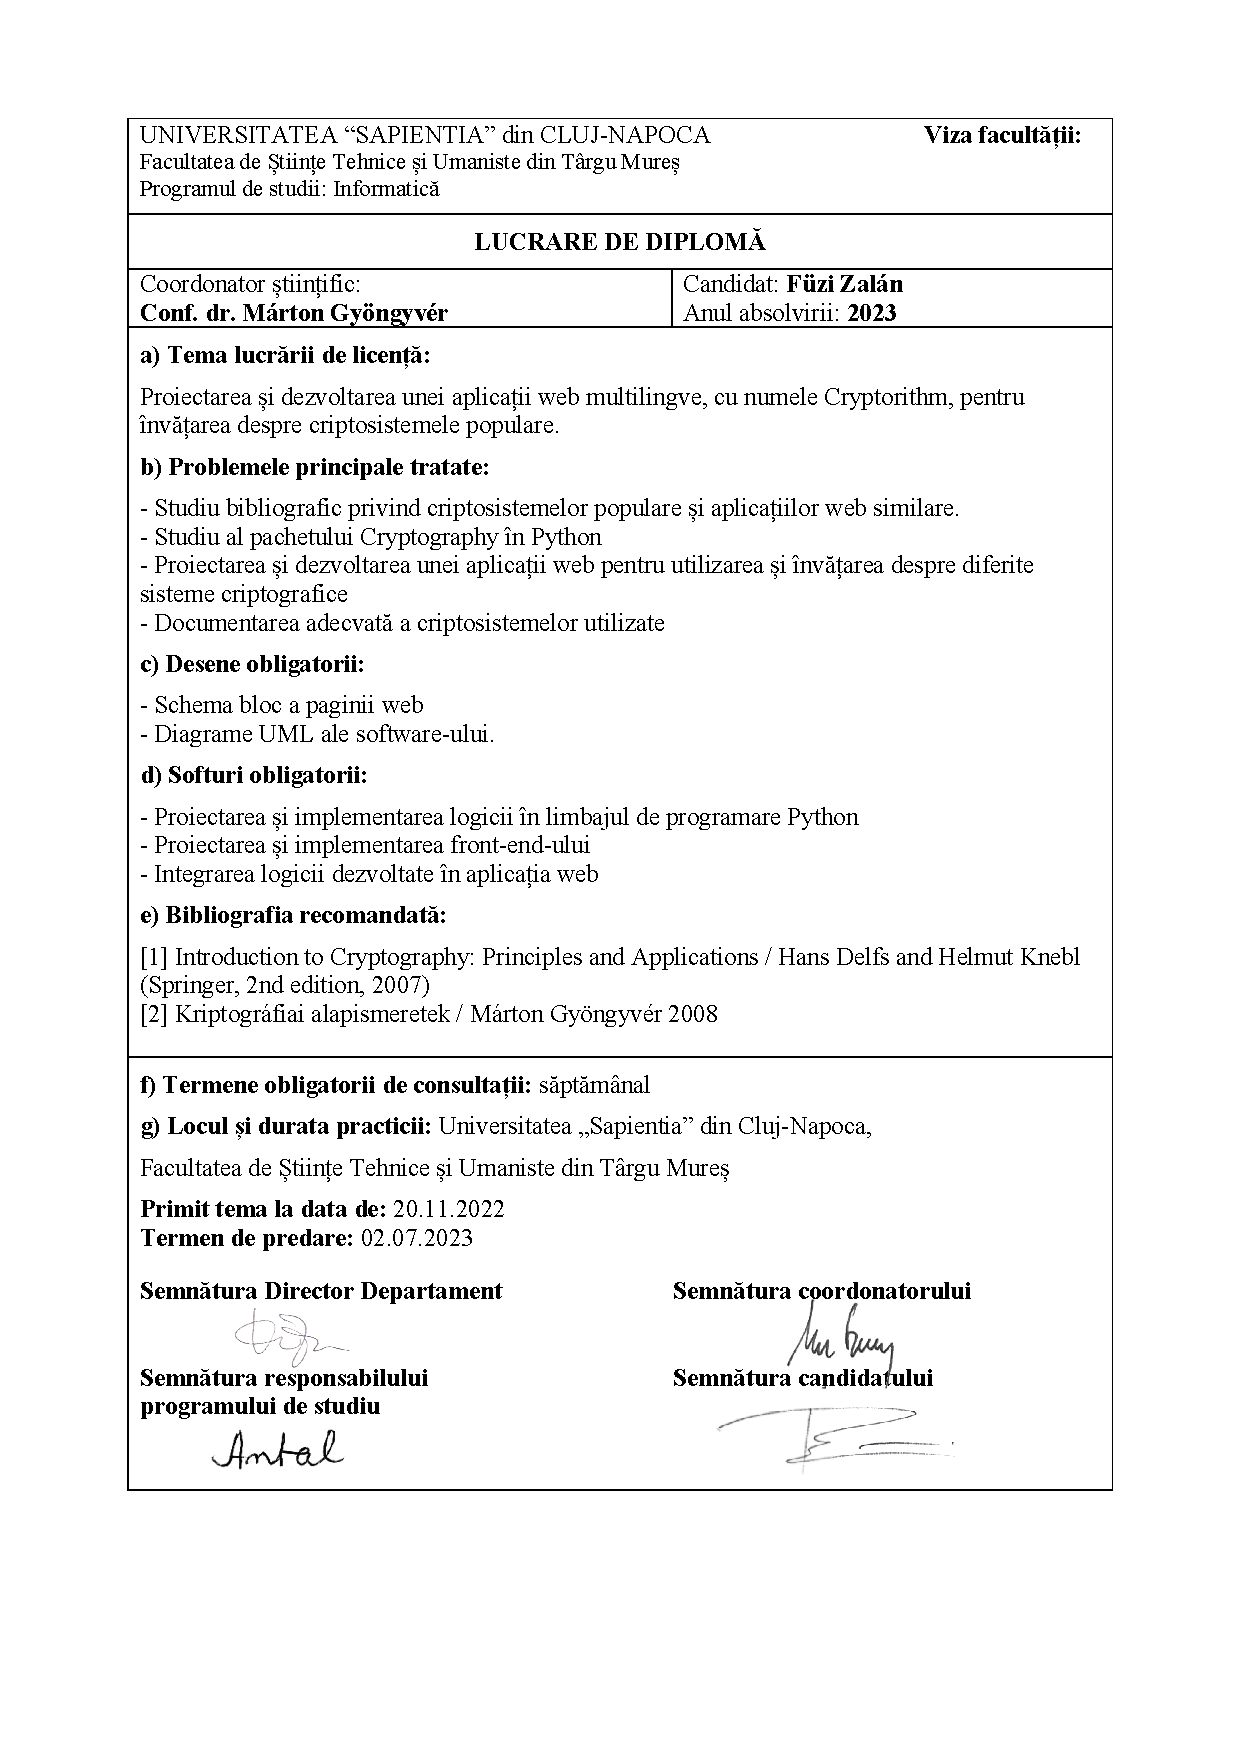
\includepdf[pages={1}]{content/Fuzi Zalan_Fisa_projectului.pdf}
	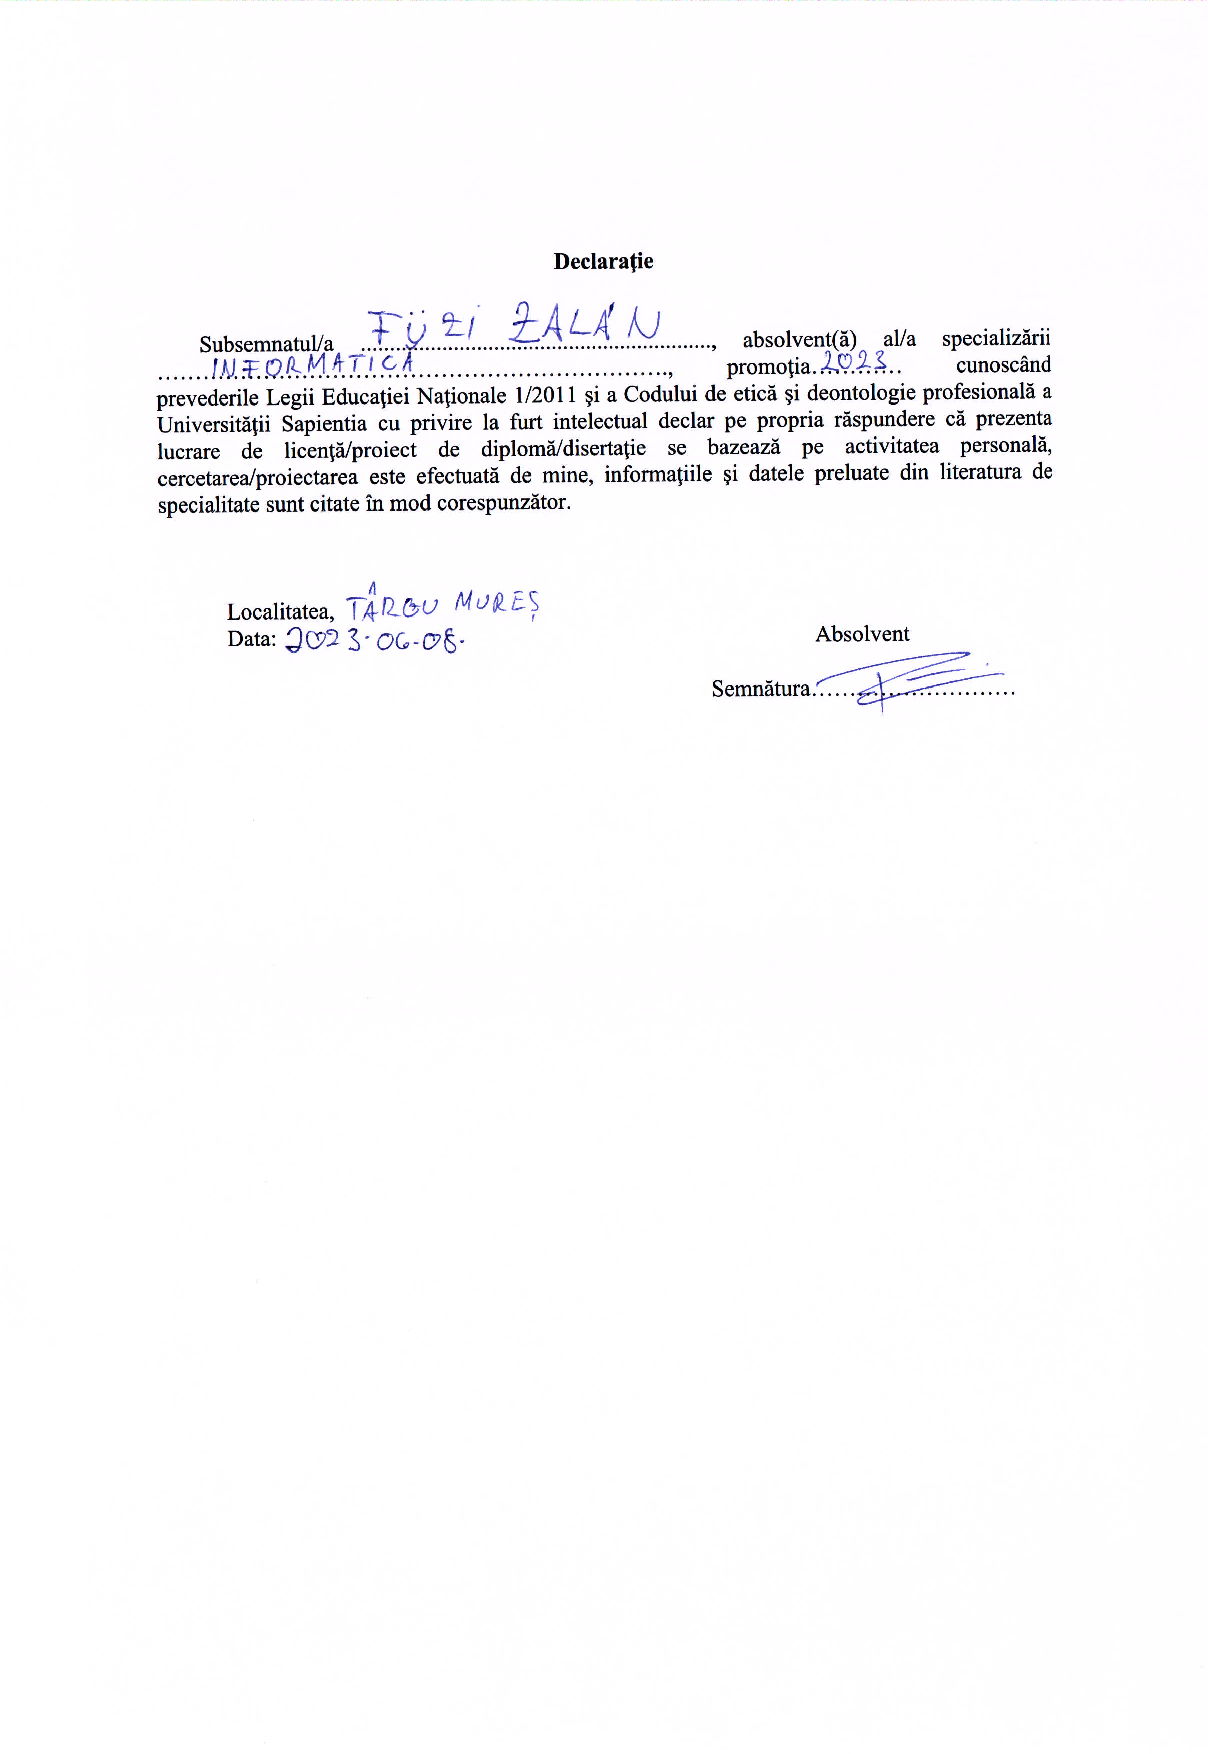
\includepdf[pages={1}]{content/Fuzi_Zalan_Declaratie_student.pdf}
	\pagenumbering{gobble}

\selectlanguage{magyar}
\hungarianParagraph

%----------------------------------------------------------------------------
% Abstract in Hungarian
%----------------------------------------------------------------------------

\chapter*{Kivonat}

A Cryptorithm egy online platform, ahol a felhasználók kriptográfiai rendszereket próbálhatnak ki, és egy kiterjedt tudásbázist kínál, hogy szabadon tanulhassanak a rendszerek eredetéről, működéséről és felhasználásáról.

A szoftver választékot kínál a népszerű és ismert módszerekből az adatok titkosításához, visszafejtéséhez és transzformációjához, lehetővé téve a felhasználóknak, hogy szabadon válogathassanak és kipróbáljanak különböző lehetőségeket. Emellett rendelkezik egy tanulói felülettel, amely hozzájárul a felhasználók számára a kriptográfiai rendszerek mélyebb megértésében. Itt információkat olvashatnak, és gyakorlati példákon keresztül sajátíthatják el ezeket a rendszereket. 

Kiemelt figyelmet fordítottam a fejlesztés során a felhasználói élmény biztosítására, így a szoftver könnyedén használható felhasználói felülettel rendelkezik. Emellett fontos szempont volt az, hogy az oldal támogassa a többnyelvűséget is, így az oldal elérhetővé válik magyar és angol nyelű felhasználók számára is.

A diplomadolgozatom további részében részletesen bemutatom a szoftver architektúráját, a megvalósított funkciókat, valamint a hozzá tartozó tudnivalókat. Emellett a felhasználói dokumentáció is részét képezi a dolgozatnak.


\vfill
\selectlanguage{romanian}

%----------------------------------------------------------------------------
% Abstract in Romanian
%----------------------------------------------------------------------------
\chapter*{Rezumat}

Cryptorithm este o platformă online unde utilizatorii pot încerca sisteme criptografice și oferă o bază de cunoștințe extinsă pentru a învăța în mod liber despre originea, funcționarea și utilizarea acestor sisteme.

Software-ul oferă o selecție de metode populare și bine cunoscute de criptare, decriptare și transformare a datelor, permițând utilizatorilor să aleagă și să încerce în mod liber diferite opțiuni. De asemenea, dispune de o interfață de învățare pentru a ajuta utilizatorii să dobândească o înțelegere mai profundă a sistemelor criptografice. Aici aceștia pot citi informații și pot învăța despre aceste sisteme prin exemple practice. 

Am acordat o atenție deosebită asigurării unei experiențe de utilizare în timpul dezvoltării, astfel încât software-ul are o interfață ușor de utilizat. În plus, a fost important ca site-ul să fie compatibil cu multilingvismul, astfel încât să fie accesibil atât pentru utilizatorii englezi, cât și pentru cei maghiari.

În restul tezei mele voi descrie în detaliu arhitectura software-ului, caracteristicile implementate și cunoștințele aferente. În plus, documentația pentru utilizatori este, de asemenea, parte a tezei.

\vfill
\selectlanguage{english}
%\englishParagraph

%----------------------------------------------------------------------------
% Abstract in English
%----------------------------------------------------------------------------
\chapter*{Abstract}

Cryptorithm is an online platform where users can try out cryptographic systems and offers an extensive knowledge base to freely learn about the origin, operation and use of these systems.

The software offers a selection of popular and well-known methods for encrypting, decrypting and transforming data, allowing users to freely choose and try out different options. It also has a learning interface to help users gain a deeper understanding of cryptographic systems. Here they can read information and learn about these systems through practical examples. 

I have paid particular attention to ensuring a user experience during development, so the software has an easy-to-use interface. In addition, it was important that the site supports multilingualism so that it is accessible to both English and Hungarian users.

In the rest of my thesis I will describe in detail the architecture of the software, the implemented features and the related knowledge. In addition, the user documentation is also part of the thesis.

\vfill
\dolgozatnyelve
\defaultParagraph
 
% Tartalomjegyzek
%~~~~~~~~~~~~~~~~~~~~~~~~~~~~~~~~~~~~~~~~~~~~~~~~~~~~~~~~~~~~~~~~~~~~~~~~~~~~~~~~~~~~~~
	\pagenumbering{arabic}
	\setcounter{page}{8}
	\tableofcontents\vfill

% A diplomadolgozat lenyegi resze
%~~~~~~~~~~~~~~~~~~~~~~~~~~~~~~~~~~~~~~~~~~~~~~~~~~~~~~~~~~~~~~~~~~~~~~~~~~~~~~~~~~~~~~

	%----------------------------------------------------------------------------
\chapter{Bevezető}%\addcontentsline{toc}{chapter}{Bevezető}
%----------------------------------------------------------------------------

A digitális korban a kriptográfia egyre növekvő jelentőséggel bír, hiszen az adatbiztonság és az adatvédelem kulcsfontosságú tényezők az információtechnológia területén. A kriptográfiai rendszerek megértése és hatékony használata elengedhetetlen az adatok titkosításához, visszafejtéséhez és biztonságos átvételéhez.

Célja a dolgozatomnak, hogy bemutassa a Cryptorithm nevű webes alkalmazást, amely egy kiterjedt platformot kínál a kriptográfiai rendszerek gyakorlati kipróbálására és tanulására. Az alkalmazás lehetővé teszi a felhasználók számára, hogy interaktív módon felfedezzék a különböző kriptográfiai algoritmusokat és azok alkalmazási területeit, mint például az SHA és Whirlpool hash fügvények, a Caesar, Affin és ChaCha20 folyamtitkosítók vagy az AES és Blowfish blokktitkosítók. Emellett a Cryptorithm egy részletes tudásbázist is nyújt, amely segíti a felhasználókat az algoritmusok eredetének, működésének és felhasználásának megértésében.

A Cryptorithm alkalmazás a Flask, egy Python alapú könnyű súlyú webes keretrendszerre épül, amely lehetővé teszi a gyors és hatékony fejlesztést. Az alkalmazás intuitív és felhasználóbarát felülettel rendelkezik, hogy könnyű legyen a navigáció és a kriptográfiai rendszerek gyakorlati alkalmazása. Az alkalmazás többnyelvű támogatást is biztosít, így bárki, függetlenül az anyanyelvétől, elérheti és használhatja a platformot.

\begin{figure}[!h]
	\centering
	
\includegraphics[scale=0.25]{images/logoCryptorithm}
	\caption{Cryptorithm logó}
\end{figure}
\pagebreak

%----------------------------------------------------------------------------
\section {Motiváció és Célkitűzések}
%----------------------------------------------------------------------------
\textbf{Kriptográfiai tudatosság növelése:}
Az alkalmazás célja, hogy növelje a felhasználók kriptográfiai tudatosságát és ismereteit. A projekt fő motivációja a felhasználók tájékozottságának növelése a digitális biztonság terén, segítve őket a kriptográfiai rendszerek megértésében és alkalmazásában.

\textbf{Gyakorlati tapasztalat nyújtása:}
Lehetőséget kapnak a felhasználók, hogy gyakorlatban is kipróbálják és megtapasztalják a kriptográfiai rendszerek működését.

\textbf{Tanulás és oktatás támogatása:}
Egy tanulói felületet van biztosítva, ahol a felhasználók elmélyülhetnek a kriptográfia terén. Motivációs tényező a tudásátadás és az oktatás támogatása, amely segít a felhasználóknak a kriptográfiai rendszerek megértésében és elsajátításában.

\textbf{Nyitottság és közösség támogatása:}
Az alkalmazás lehetőséget nyújt az idegen anyanyelvű felhasználóknak is a használatra, hogy bővítsék tudásukat a kriptográfiai rendszerekről.







	%----------------------------------------------------------------------------
\chapter{Programok, technológiák bemutatása} \label{fejezet2}
%----------------------------------------------------------------------------

\section {Az alkalmazás felépítése}

\subsection{Frontend}

A frontend fejlesztéséhez HTML-t, CSS-t és JavaScriptet  (\ref{fig:logosFront}) használtam, amelyek lehetővé teszik az interaktív felhasználói felület létrehozását és a dinamikus funkcionalitás implementálását. Ezek a technológiák biztosítják a felhasználók számára az intuitív böngészési élményt és a kriptográfiai rendszerek kipróbálását.
Valamint a Jinja2 sablonmotort használtam, hogy segítsen a dinamikus tartalmú weboldalak generálásával, amelynek használatát egy külön szekcióban fejtem ki. (\ref{sec:jinja2})

\textbf{HTML:}
Egy szabványosított jelölőnyelv, amelyet a weboldal strukturálására és tartalma megjelenítésére használtam. Segítségével definiáltam az elemeket, például címeket, szövegeket, képeket, hivatkozásokat stb.

\textbf{CSS:}
Egy stílusleíró nyelv, amelyet a weboldal megjelenítési formázására használtam. Azáltal, hogy különböző stílusokat és tulajdonságokat adtam meg az elemeknek, mint például a szín, a betűtípus, a méret, a margók, a pozíció stb., a CSS lehetővé tette a weboldal testreszabását és a vizuális vonzereje növelését.

\textbf{JavaScript:}
Egy programozási nyelv, amelyet az alkalmazás interaktív funkcióinak megvalósítására használtam. A JavaScript lehetővé teszi a weboldalam dinamikus működését, a felhasználói interakciókat, az adatok feldolgozását és a weboldalhoz kapcsolódó események kezelését.

\begin{figure}[!h]
	\centering
	
\includegraphics[scale=0.3]{images/logoHtmlCssJs}
	\caption{HTML - CSS - JS logók}
	\label{fig:logosFront}
\end{figure}


\newpage
\subsection{Backend}

Backend oldalon a szerveroldali programozáshoz a Python programozási nyelvet választottam, amely nagy népszerűségnek örvend Flask keretrendszerrel kombinálva. A Python és a Flask együtt lehetővé teszik a hatékony és gyors fejlesztést, valamint az API-k létrehozását és a kérések kezelését.

Az adatbázis kezeléséhez az SQLAlchemy nevű Python könyvtárat használtam, melynek segítségével könnyedén lehet adatmodelleket definiálni és adatbázisműveleteket végezni. Ezáltal hatékony és strukturált adatkezelést biztosít az alkalmazásban.

Ezen technológiák kombinációja lehetővé teszi az alkalmazás teljeskörű működését, az interaktív felhasználói felülettől kezdve az adatok kezeléséig és tárolásáig. Az alkalmazás fejlesztése során a modern frontend és backend technológiák összekapcsolása révén egy hatékony és felhasználóbarát környezetet hoztam létre a kriptográfiai rendszerek kipróbálásához és tanulásához.  (\ref{fig:logosBack})

\vspace{10pt}
\textbf {Python:}
A Python egy magas szintű programozási nyelv, amelyet egyszerű és olvasható szintaxisa jellemez. A Python nagyon rugalmas és sokoldalú, és széles körben használják a webfejlesztés, adatelemzés, mesterséges intelligencia, gépi tanulás és sok más területen. A Pythonban kifejezőerő és kényelem találkozik, ami lehetővé teszi a gyors és hatékony fejlesztést. Emellett a Python gazdag könyvtárökoszisztémával rendelkezik, amely számos előre elkészített funkcióval és modullal bővíti a fejlesztési lehetőségeket.

\vspace{10pt}
\textbf {Flask:}
A Flask egy könnyűsúlyú és rugalmas webes keretrendszer Pythonban. A Flask lehetővé teszi a webalkalmazások gyors és hatékony fejlesztését, minimális konfigurációval és egyszerű szintaxisával. A Flask kiváló választás olyan projektekhez, amelyek kisebb méretűek vagy kevesebb komplexitást igényelnek, ugyanakkor rugalmasságot és skálázhatóságot biztosítanak. A Flask lehetőséget nyújt a beépített funkciók, mint például útvonalak, nézetek, sablonok és adatbázis kezelése egyszerű implementálására.

\vspace{10pt}
\textbf {SQLAlchemy:}
Az SQLAlchemy egy Python alapú ORM (Object-Relational Mapping) keretrendszer, amely lehetővé teszi az adatbázisokhoz való könnyű és hatékony hozzáférést. Az ORM segítségével a fejlesztők Python objektumokat tudnak kezelni és manipulálni, miközben azokat az adatbázisban tárolják. Ezáltal az SQLAlchemy elrejti az adatbázis-specifikus részleteket és absztrakciós réteget biztosít a programozó számára.

\pagebreak
\begin{figure}[!h]
	\centering
	
\includegraphics[scale=0.15]{images/logoPythonFlaskSqlalchemy}
	\caption{Python - Flask - SQLAlchemy logók}
	\label{fig:logosBack}
\end{figure}


\section {Hasonló platformok, szoftverek összehasonlítása}

\textbf{Cryptii \cite{Cryi}:} A Cryptii egy online titkosítási és dekódolási weboldal, amely algoritmusok széles skáláját támogatja. Különböző szimmetrikus és aszimmetrikus titkosítási algoritmusok közül választhat. A weboldal emellett lehetőséget biztosít a kódolásra, a hashelésre és a tömörítésre is. A bevitel és kimenet között lehetőség van különböző rétegeket beiktatni, így a két végpont között több algoritmus is alkalmazható.

\textbf{Encode-Decode \cite{EnDe}:} Az Encode-Decode egy olyan weboldal, amely különböző algoritmusokhoz kínál titkosítási és dekódolási szolgáltatásokat. A weboldal egy egyszerű felületet biztosít, ahol beírhatja a szöveget, és kiválaszthatja a kívánt titkosítási vagy visszafejtési módszert.

A Cryptii és Encode-Decode platform sem ad leírást a használt algoritmusokról, így ezeket csak úgy lehet hatékonyan használni amennyiben ismerjük azokat, vagy más forrásokból tájékozódunk róluk.

\vspace{10pt}
\textbf{CyberChef \cite{CyCh}:} A CyberChef egy hatékony online eszköz az adatmanipulációhoz és a titkosításhoz/dekódoláshoz. A műveletek széles skáláját kínálja, beleértve az olyan titkosítási algoritmusokat, mint az AES, RSA, XOR és még sok más. Támogatja továbbá a kódolást, a hashelést, a tömörítést és más adattranszformációkat.

\textbf{Rumkin \cite{Rum}:} A Rumkin egy olyan weboldal, amely kriptográfiai eszközök széles gyűjteményét kínálja. Különböző algoritmusokhoz kínál lehetőségeket, mint például a Caesar rejtjelezés, a Rail Fence rejtjelezés, a Playfair rejtjelezés és még sok más. Emellett kódolásra, hashelésre és steganográfiára szolgáló eszközöket is tartalmaz.

\textbf{dCode \cite{dCo}:} A dCode egy olyan online platform, amely titkosítási és dekódolási eszközök hatalmas gyűjteményét kínálja. Algoritmusok, titkosítások és kódolások széles skáláját fedi le, beleértve a klasszikus titkosításokat, modern titkosítási módszereket és speciális kódolásokat. Emellett kriptoanalízishez is kínál eszközöket.

Az utolsó három alkalmazás esetében már több, részletesebb leírást lehet kapni az algoritmusokról, bár már kevésbé felhasználóbarátok, mint az első két platform.



	%----------------------------------------------------------------------------
\chapter{Kriptográfiai alapok és rendszerek}
%----------------------------------------------------------------------------


\section{Kriptográfiai alapfogalmak}
A Cryptorithm rendszer használata során néhány alapvető kriptográfiai fogalom ismerete előnyös lehet. Az alábbiakban néhány ilyen fogalmat tisztázok, amelyek segíthetnek a rendszer hatékony használatában.
\subsection{Titkosítás}
A titkosítás olyan folyamat, amely során az eredeti üzenetet (nyílt szöveget) átalakítjuk egy titkosított formává, hogy csak a jogosultak tudják elolvasni. Az alkalmazásban található kriptográfiai rendszerek segítségével a felhasználók titkosíthatnak és visszafejthetnek üzeneteket.

\subsection{Kulcs}
A kulcs a kriptográfiában egy olyan titkosítási vagy visszafejtési folyamat során használt információdarab, amely alapvetően befolyásolja a kriptográfiai algoritmus működését és a végeredményt. Biztosítják az adatok biztonságát és védelmet nyújtanak a jogosulatlan hozzáférésekkel szemben. Ugyanakkor fontos megjegyezni, hogy az erős és biztonságos kulcs kiválasztása és ennek tárolása, kezelés elengedhetetlen a megfelelő kriptográfiai rendszerek kialakításában.

\newpage
\subsection{Titkosítási módok}
A titkosítási módok meghatározzák, hogy a titkosítás hogyan történik az üzenetek blokkjainak kezelése során. A gyakran használt titkosításí módok a következőek: ECB(Electronic Codebook), CBC(Ciper Block Chaining), CFB(Cipher Feedback), OFB(Output Feedback) és a CTR(Counter).
A felsorolt üzemmódok mellett számos más speciális üzemmód létezik, amelyek különböző funkciókkat és jellemzőket kínálnak. A megfelelő kiválasztása és alkalmazása az adott kriptográfiai algoritmustól függ.

A Cryptorithm esetében az AES blokk titkosító CTR üzemmódban próbálható ki, ami azt jelenti, hogy a blokkok titkosítása egy folyamatosan növekvő számláló alapján történik. A számláló értékét XOR-olják az adatblokkal a blokk titkosítása előtt. Ez a módszer párhuzamosításra alkalmas, mivel a blokkok függetlenül titkosíthatóak.

\subsection{Rejtjelezések}
A dolgozatomban 2 fajta rejtjelezést, avagy tikosítást különböztetek meg, a \textbf{klasszikus} és a \textbf{szimmetrikus} titkosítókat. A klasszikus titkosítókhoz tartoznak a Caesar és Affin rejtjelezések, ezeket a rendszereket ma már csak kizárólag példaképpen használják a bevezetéshez a kriptográfia világába. A szimmetrikus titkosítás az jelenti, hogy mind a titkosításra, mind a visszafejtésre ugyanazt a kulcsot használják, ide tartoznak a ChaCha20, az AES és a Blowfish rejtjelezések. Továbbá mindegyik rejtjelezés két féle lehet, blokk- vagy folyamtitkosító.

A \textbf{blokktitkosítók} a bemeneti adatot blokkokra osztják, majd ezeket a blokkokat titkosítják. A blokkok mérete álltalában azonos, és ugyanazt a titkosítási kulcsot és algoritmust használják. Ilyen titkosító például az AES és a Blowfish. Előnyei a hatékonyság, mivel a blokkok egyszerre titkosíthatóak és dekódolhatóak, továbbá hibajavítási képessége, mert egy hibás blokk nem terjed át a többi blokkra.

A \textbf{folyamtitkosítók} bitenként vagy bitek kis csoportjaival dolgozik, és a titkosítás során egy folyamot generál. A folyamtitkosítás az adatokat a generált kulcs folyammal kombinálja. Előnyei közé tartozik a sebesség és az adatfolyam feldolgozásának hatékonysága, mivel az adatokat bitek szintjén lehet titkosítani és dekódolni. Emellett a folyamtitkosítás ellenállóbb lehet a blokktitkosítással szembeni kriptoanalitikai támadásokkal szemben, mivel nem állít elő azonos bemenetekhez azonos kimeneteket. Ilyen titkosító például a ChaCha20.

\pagebreak
\subsection{Hash függvények}
Az alkalmazás a rejtjelezők mellett még lehetőséget ad a hash függvények tanulmányozására is. A hash-függvények olyan matematikai algoritmusok, amelyek egy tetszőleges hosszúságú bemenetet (pl. üzenetet) átalakítanak egy fix hosszúságú, látszólag véletlenszerű kimenetbe. A hashelés segít a felhasználóknak az adatok hitelességének ellenőrzésében. Továbbá erejük és megbízhatóságuk abban rejlik, hogy irreverzibilisek, nem lehet visszaállítani a hash értékéből a bemeneti adatot eredeti formájában és ugyanakkor ütközmentesek, vagyis nagyon alacsony valószínűséggel található két különböző bemenet, amelyek ugyanahhoz a hash értékhez vezetnek. Ilyen függvény például az SHA, a Whirlpool és a bcrypt.


\section{Kriptográfia rendszerek}
A következőkben megemlítem azokat a krpitográfiai módszereket amelyek elérhetőek a Cryptorithm alkalmazásban.


\subsection{Klasszikus titkosítók bemutatása}
A \textbf{Caesar} rejtjelezés Julius Caesarról, az ókori római katonai és politikai vezetőről kapta a nevét, aki a feltételezések szerint ezt a titkosítási technikát használta. Egy egyszerű eltolásos titkosítási módszer, amelyben az összes betűt egy adott számmal, a kulcsként használt eltolással helyettesítik. Például, ha a kulcs 3, akkor az "A" betűt a "D" betűre cserélik, a "B" betűt az "E" betűre stb. A Caesar rejtjelezés könnyen feltörhető, mivel csak 26 lehetséges eltolási kulcs létezik, amelyeket egyszerűen végig lehet próbálni.


Az \textbf{Affin} rejtjelezés egy egyszerű szubsztitúciós rejtjelezési módszer, amely a Caesar rejtjelezésre épül. Az Affin rejtjelezés egy lineáris transzformációt alkalmaz a betűkön, amely egy egyenlet alapján helyezi át azokat. Az Affin rejtjelezés a kulcsként használt két paraméter segítségével végez transzformációt az üzeneten. Az Affin rejtjelezés gyenge pontja, hogy az egyszerű frekvenciaanalízis módszerekkel feltörhető lehet, különösen kis méretű kulcsok esetén.


Fontos megjegyezni, hogy az Affin és Caesar rejtjelezések gyakorlati alkalmazásban már nem számítanak biztonságosnak, mivel könnyen feltörhetők.

\pagebreak
\subsection {Szimmetrikus titkosítók bemutatása}
A \textbf{ChaCha20} elsősorban szimmetrikus titkosítási algoritmusként és folyamtitkosítóként használatos. Gyakran alkalmazzák hálózati protokollokban, biztonságos kommunikációban és nagy teljesítményű titkosítást igénylő alkalmazásokban. A ChaCha20 a sebességéről és biztonságáról ismert, és a régebbi titkosítók, például az RC4 alternatívájaként vált népszerűvé. \cite{Heiko}


Az \textbf{AES} egy szimmetrikus blokktitkosítási algoritmus, amelyet a biztonságos adatátvitel és tárolás céljából használnak. Az AES algoritmus blokkokat titkosít a bemeneti üzenetből, és ezek a titkosított blokkok kombinálódnak a kimeneti titkosított üzenet létrehozásához. Az AES-t az Egyesült Államok Kormánya ajánlja a kormányzati és ipari alkalmazásokban. Az AES több különböző kulcsmérettel (128, 192, 256 bites) és különböző üzemmódokkal (pl. CTR, CBC, ECB) használható. \cite{AES}


A \textbf{Blowfish} egy szimmetrikus kulcsú blokktitkosító, amely 64 bites blokkokkal dolgozik, és változó kulcsméreteket támogat (32 bittől 448 bitig). Gyakran használják olyan alkalmazásokban, amelyek érzékeny adatok titkosítását és visszafejtését igénylik. A Blowfish-t széles körben alkalmazzák protokollokban, szoftverekben és hardveres rendszerekben a titkosság és az adatvédelem biztosítása érdekében. \cite{Blowfish}


\subsection {Hash függvények bemutatása}
A \textbf{Whirlpool} egy hash-függvény, amelyet általában adatintegritás-ellenőrzésre és digitális aláírásra használnak. Fix méretű, jellemzően 512 bit hosszú hash-értéket állít elő. A Whirlpoolt különböző biztonsági alkalmazásokban használják, például a fájlok integritásának ellenőrzésére, jelszavak tárolására és üzenethitelesítésre. \cite{Whirlpool}

Az \textbf{SHA} egy hash függvény család, amelyeket a digitális adatok integritásának ellenőrzésére és az adatok egyedi azonosítására használnak. Az SHA hash függvények, például az SHA-1, SHA-256 stb., egy adott bemeneti üzenetet átalakítanak egy fix hosszú hash kóddá. Az SHA algoritmusok irreverzibilisek, vagyis a hash értékből nem lehet visszaállítani az eredeti üzenetet. Ez a tulajdonságuk hasznos a jelszavak, digitális aláírások és az üzenetek integritásának védelmében.

A \textbf{bcrypt} egy hash függvény, amelyet leginkább jelszavak biztonságos tárolására és ellenőrzésére használnak. Az algoritmus tervezésekor arra törekedtek, hogy lassú legyen a hash függvények hasítási sebessége, hogy megnehezítse a jelszavak visszafejtését a hash értékből. Az algoritmus egy sor iterációt végez a jelszó hasításához, és egy só (salt) értéket használ, amely tovább növeli a biztonságot. A jelszó karakterlánc, egy számokban kifejezett költség és egy sóérték a bcrypt algoritmus bemenete. Ezeket a bemeneteket a bcrypt függvény egy 24 bájtos (192 bites) hash létrehozására használja. \cite{bcrypt}

\section{Feltörési módszerek}
A kriptográfia algoritmusok célja, hogy megvédjék az adatokat az illetéktelen hozzáféréstől. Azonban az informatikai fejlődéssel és az idő múlásával párhuzamosan megjelentek bizonyos feltörési módszerek is, melyeknek célja, hogy az adatokat megpróbálják visszafejteni eredeti, bemeneti formájukra. Az alábbiakban bemutatok néhány gyakran használt kriptográfiai fetörési módszert:

\begin{itemize}
	\item\textbf{Brute force:} Ez a módszer az összes lehetséges kulcs kipróbálását jelenti, amíg megtaláljuk a helyes kulcsot. Bár hatékony kriptográfiai algoritmusok esetén ez időigényes és gyakran megvalósíthatatlan feladat, bizonyos esetekben hatékony lehet.

	\item\textbf{Frekvenciaanalízis:} Ez a módszer az adott nyelven használt betűk gyakoriságának elemzésén alapul. A gyakrabban előforduló betűk azonosítása segíthet a titkosított szöveg visszafejtésében, különösen, ha az adott nyelvre jellemző mintázatokat lehet azonosítani. Bizonyos algoritmusok esetében ez teljesen kivitelezhetetlen mivel a titkosított szövegben nincsen nyelvi jellegű információ, amely alapján ki lehetne használni a betűk gyakoriságát.
\end{itemize}




































	%----------------------------------------------------------------------------
\chapter{Szoftver}
%----------------------------------------------------------------------------

\section{Felhasználói követelmények}

\textbf{Regisztráció és bejelentkezés:} Lehetőséget van regisztrációra az alkalmazásban, amely után a felhasználók bejelentkezhetnek a személyes fiókjukba. Ez lehetővé teszi számukra a mentett adatokhoz való hozzáférést.

\textbf{Kriptográfiai rendszerek kiválasztása:} Különböző kriptográfiai rendszerek elérhetőek, amelyeket bejelentkezés után lehet kipróbálni. Ehhez megjelenik egy menüt, ahol kényelmesen navigálhatnak a rendszerek között.

\textbf{Rendszerek kipróbálása és tesztelése:} A felhasználóknak lehetősége van arra, hogy kipróbálják és teszteljék a választott kriptográfiai rendszereket. Ehhez felhasználóbarát és interaktív felületet van biztosítva, ahol megadhatják a bemeneti adatokat, és láthatják a kimeneti eredményeket.

\textbf{Tanulási anyagok és információk elérhetősége:} Az alkalmazásnak tartalmaz egy tanulói felületet , ahol a felhasználók elérhetik a kriptográfiai rendszerekhez kapcsolódó részletes információkat és példafeladatokat. Ennek az oldalnak az eléréséhez nem szükséges a bejelentkezés.

\textbf{Nyelvi támogatás:} Az alkalmazás lehetőséget ad a felhasználóknak arra, hogy különböző nyelveken használják az alkalmazást. Ehhez egy egyszerű nyelv kiválasztó van biztosítva, amely lehetővé teszi a felhasználóknak a kívánt nyelv kiválasztását. A nyelvek rövidítve, ISO 639.1-es kódjuk szerint vannak feltüntetve.

\newpage
\section{Rendszerkövetelmény}
A Cryptorithm rendszerkövetelménye funkcionális és nem funkcionális részekre oszlik. A funkcionális része tartalmazza az alkalmazás fő céljait és funkcionalitását, hogy hogyan kéne működjön a rendszer és milyen lehetőségei vannak a felhasználónak, míg a nem funkcionális rész kitér a rendszerrel szemben támasztott követelményekre, mint például a felhasználói élmény, többnyelvűség és a rendszer architektúrája.

\subsection{Funkcionális}
\textbf{Kriptográfiai eszközök:} Az alkalmazás választékot kínál a népszerű és ismert eszközökből az adatok titkosításához, visszafejtéséhez és transzformációjához. A felhasználók szabadon válogathatnak és kipróbálhatnak különböző lehetőségeket.

\textbf{Tanulói felület:} Az alkalmazás rendelkezik egy tanulói felülettel, ahol a felhasználók elmélyülhetnek a kriptográfiai rendszerek megértésében. Itt információkat olvashatnak és gyakorlati példákon keresztül elsajátíthatják ezeket a rendszereket.

\textbf{Többnyelvűség:} Az alkalmazás támogatja a többnyelvűséget, így elérhetővé válik idegen nyelvű felhasználók számára is. A felhasználók kiválaszthatják az anyanyelvüket vagy egyébb preferált nyelvet az alkalmazás használatához.

\textbf{Visszajelzés:} Amennyiben ismert kivétel keletkezik a rendszserben ezt felugró üzeneten keresztül van leközölve, ami ismerteti a hibát. Kivétel keletkezhet nem megfelelő beviteli adatok nyomán, például rossz vagy nem megfelelő kulcsméret megadása, vagy olyan oldalra való navigáció ahova a felhasználónak nincsen jogosultsága. Az előző esetet a hibának megfelelő üzenettel közlődik, míg utóbbi egy az érvényben levő jogosultságnak megfelelő oldalra navigálja a felhasználót.

\textbf{Szerepkörök:} A rendszert két fajta felhasználó számára elérhető, bejelentkezett és nem bejelentkezett. A bejelentkezett felhasználónak elérhető a weboldal összes funkcionalitása, ezzel szemben a nem bejelentkezett felhasználó nem jogosult a kriptográfia rendszerek használatára.

\begin{figure}[!h]
	\centering
	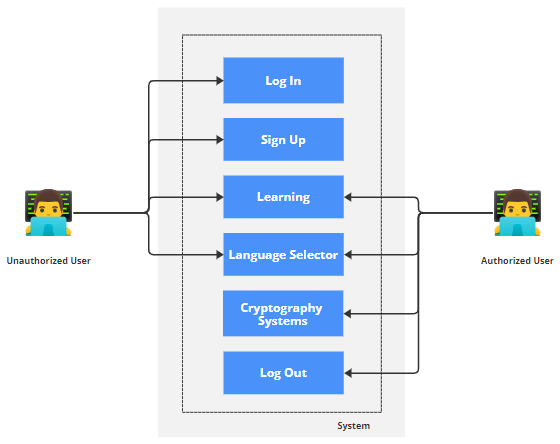
\includegraphics[scale=0.6]{images/UseCaseDiagram}
	\caption{Use case diagram}
\end{figure}


\newpage
\subsection{Nem funkcionális}

\begin{itemize}
	\item\textbf{Felhasználói élmény:} Az alkalmazás könnyen használható felhasználói felülettel rendelkezik. Az intuitív navigáció és a felhasználóbarát tervezés lehetővé teszi a felhasználók számára a könnyű kezelést és a zökkenőmentes interakciót az alkalmazással. Továbbá megfelelő felugró üzenetekkel jelez vissza a rendszer minden művelet elvégzése után.

	\item\textbf{Teljesítmény:} Az alkalmazás működése gyors és hatékony.

	\item\textbf{Biztonság:} Felhasználói adatok védve vannak, megfelelően vannak tárolva.

	\item\textbf{Skálázhatóság:} Az alkalmazás képes kezelni a megnövekedett felhasználói forgalmat és rugalmasan skálázódni.

	\item\textbf{Hibatűrés:} Hibakezelés és hibajavítás mechanizmusainak megléte, az alkalmazás ellenálló képessége van a hibákhoz. Redszer leállás esetén az újraindítás nem időigényes.

	\item\textbf{Reszponzívitás:} A weboldal felülete főként asztali számítógépekre, laptopokra van optimalizálva, továbbá támogatja a népszerű böngészőket.
\end{itemize}

\begin{figure}[!h]
	\centering
	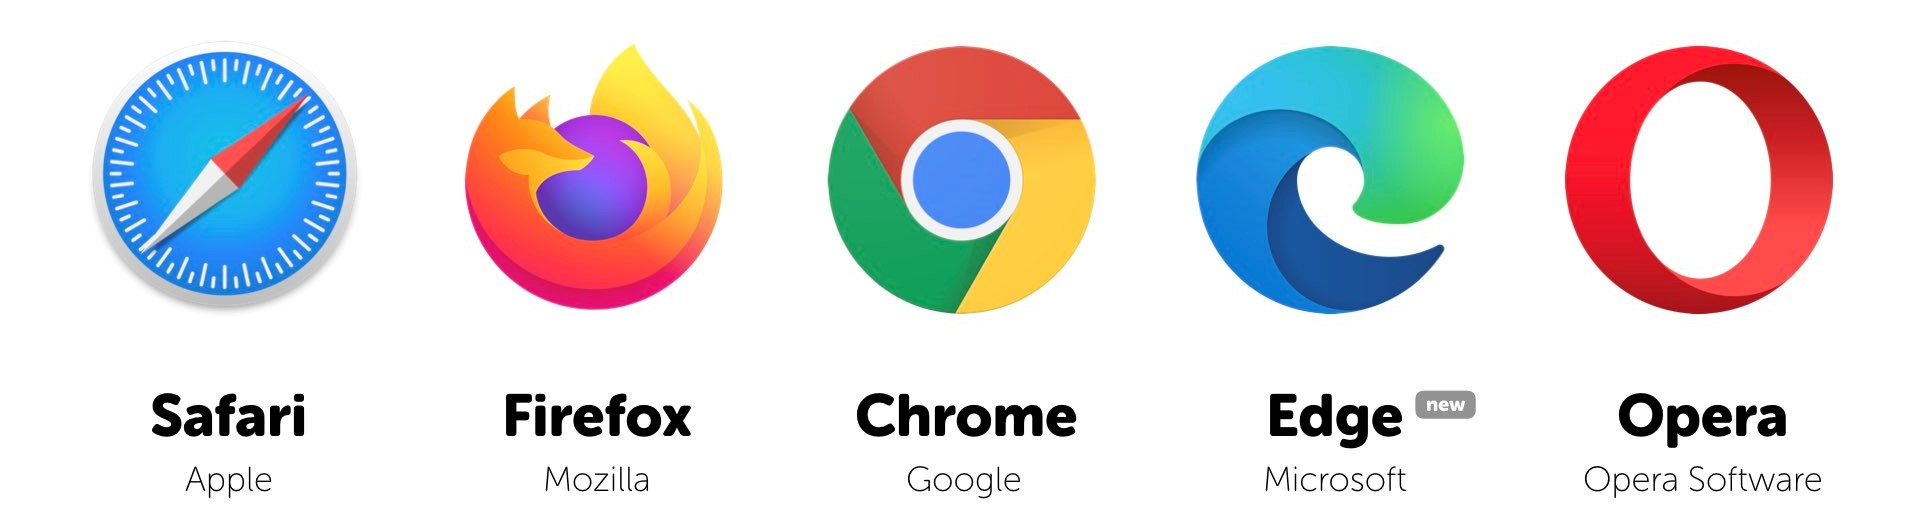
\includegraphics[scale=0.12]{images/webBrowsers}
	\caption{Népszerűbb Böngészők}
\end{figure}

\newpage
\section{A rendszer architektúrája}
Az alkalmazás architektúrája a következő komponenseket kombinálja, hogy a felhasználók kényelmesen használhassák a Cryptorithm alkalmazást. A felhasználói interfész réteg lehetővé teszi a felhasználók interakcióját az alkalmazással, az üzleti logika réteg hajtja végre a szükséges műveleteket és feldolgozza a kéréseket, míg az adatbázis réteg biztosítja az adatok tartós tárolását és kezelését. Az architektúra segít a rendszer komponenseinek szétválasztásában és a fejlesztés hatékonyságának növelésében.

\begin{figure}[!h]
	\centering
	\includegraphics[scale=0.23]{images/RendszerArchitektúra}
	\caption{Rendszer Architektúra}
\end{figure}

\textbf{Felhasználói interfész:} Ez a rész felelős az alkalmazás felhasználói felületének megjelenítéséért és a felhasználóval való interakcióért. Megvalósítása az alkalmazásban HTML, CSS és JavaScript segítségével van kivitelezve. Ez a réteg jeleníti meg a kriptográfiai rendszerek kiválasztására, tesztelésére és a tanulói anyagokhoz való hozzáférésre szolgáló felületeket.

\textbf{Üzleti logika:} Az üzleti logika réteg felelős az alkalmazás működéséért, a felhasználók által végrehajtott műveletek feldolgozásáért és az eredmények előállításáért. Itt találhatóak a szerveroldali Python fájlok, amelyek a kriptográfiai műveletek, adatfeldolgozás és adatbázis-interakciók végrehajtásáért felelősek. Flask keretrendszert használva ez a réteg kezeli a HTTP kéréseket és válaszokat.

\textbf{Adatbázis:} Az alkalmazás adatbázisában tárolódnak a felhasználói adatok, például a regisztrált felhasználók adatai és előzményei. Az adatbázis kezelésére az SQLAlchemy Python könyvtárat használtam, amely lehetővé teszi a könnyű adatbázis-műveletek végrehajtását és az adatmodell definiálását.



	%----------------------------------------------------------------------------
\chapter{Tervezés és megvalósítás}
%----------------------------------------------------------------------------

A projektet Visual Studio Code segítségével fejlesztettem, amely egy ingyenes és nyílt forráskódú fejlesztői környezet. Bár alapvetően könnyűsúlyú, ennek ellenére erőteljes szövegszerkesztő, mivel számos programozási nyelvet és technológiát kínál. A telepítése után nagyban testreszabhatjuk saját igényeink szerint és számos egyébb funkciókhoz juthatunk a bővítmények telepítésével.

6 részre bontottam a projektet: instance, cryptorithms, languages, static, templates, cryptorithm 

\begin{itemize}
	\item\textbf{Instance}:
Az instance mappában van eltárolva az adatbázis lokálisan, melynek modelje a models.py fájlban van definiálva.

	\item\textbf{Cryptorithms}:
A cryptorithms mappában levő fájlokban kerültek kivitelezésre és implementálásra a kriptográfiai rendszerek.

	\item\textbf{Languages}:
A nyelvekért felelős .json kiterjesztésű fájlok itt vannak tárolva, itt van egy meghatározott struktúrában lefordított tartalma az oldalnak.

	\item\textbf{Static}:
A static alatt a .css és .js fájlok kerültek létrehozásra, melyek a weboldal dizájnért felelősek.

	\item\textbf{Templates}:
A template mappába kerültek az alap .html fájlok amelyek a tartalom megjelenitéséért felelősek.

	\item\textbf{Cryptorithm}:
A fő mappa a Cryptorithm amely magába foglalja az előbb említett részeket, valamint az API kéréseket és válaszokat, a szessziókezeléshez, a projekt inicializálásához szükséges fájlokat, továbbá az adatbázis adatmodelljét és a projektet indító main fájlt.

\end{itemize}

\begin{figure}[!h]
	\centering
	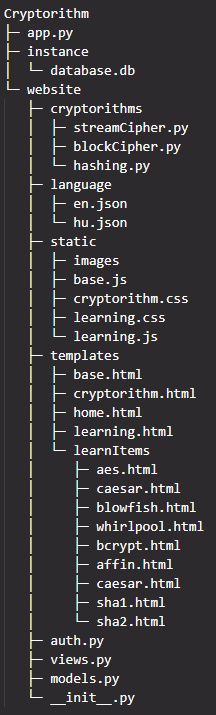
\includegraphics[scale=0.9]{images/fájlStruktúra}
	\caption{Rendszer fájl struktúrája}
\end{figure}

\section {Könyvtárak}
A következőekben bemutatom a jelentősebb Python könyvtárakat, melyek segítettek az alkalmazás implementálásában.

\begin{itemize}
  	\item\textbf{Cryptography:}
Kriptográfiai funkciókat és algoritmusokat kínál. Ez a könyvtár ideális választás a projektben, mivel számos kriptográfiai műveletet valósíthatunk meg vele. A Cryptography megbízható és jól dokumentált eszköz a kriptográfiai műveletek biztonságos végrehajtásához. Ennek a könyvtárnak a segítségével lett kivitelezve az AES rendszer.

 	 \item\textbf{Flask:}
A projektben a Flask keretrendszert használom a webes alkalmazás felépítéséhez és a kérések kezeléséhez. A Flask könnyen tanulható és rendkívül rugalmas, ami lehetővé tette, hogy könnyedén kialakítsam a vágyott funkciókat és testreszabhasam az alkalmazást.

A következő kódrészlet a tanulói oldal betöltésének kérését mutatja be:
\begin{lstlisting}[caption={Learning oldal renderelése}, captionpos=b, language = Python]
@views.route('/learning/<language>', methods=['GET', 'POST'])
def learning(language):
    if(language not in languages):
        language = app_language
    return render_template("learning.html", user=current_user, language=language, **languages[language])
\end{lstlisting}

 	 \item\textbf{FlaskSQLAlchemy:}
A FlaskSQLAlchemy egy könnyen használható és hatékony ORM (Object-Relational Mapping) könyvtár, amely lehetővé teszi az adatbázis műveletek kezelését a Flask alkalmazásban. Az SQLAlchemy révén a FlaskSQLAlchemy segít az adatbázis kapcsolatok kezelésében, az adatmodell osztályok definiálásában és az adatbázis műveletek végrehajtásában. A FlaskSQLAlchemy használata átlátható és hatékony adatbázis-interakciókat tesz lehetővé a projektben.

A következő kódrészlet az adatbázis modellek implementálását mutatja be:
\begin{lstlisting}[caption={Adatbázis modellek}, captionpos=b, language = Python]
class User(db.Model, UserMixin):
    id = db.Column(db.Integer, primary_key=True)
    email = db.Column(db.String(150), unique=True)
    password = db.Column(db.String(150))
    first_name = db.Column(db.String(150))
    datas = db.relationship('Data')

class Data(db.Model):
    id = db.Column(db.Integer, primary_key=True)
    data = db.Column(db.String(10000))
    cryptype = db.Column(db.String(100))
    paramA = db.Column(db.String(100), nullable=True)
    paramB = db.Column(db.String(100), nullable=True)
    user_id = db.Column(db.Integer, db.ForeignKey('user.id'))
\end{lstlisting}

\pagebreak
 	 \item\textbf{FlaskLogin:}
A FlaskLogin egy hasznos kiegészítő a Flask keretrendszerhez, amely segít az autentikáció és az azonosítás kezelésében a webes alkalmazásban. Ennek segítségével egyszerűen implementálhattam a felhasználói regisztrációt, bejelentkezést és kijelentkezést a rendszerben. Ez a könyvtár felelős a felhasználói munkamenetek és a hozzáférési jogosultságok kezeléséért.

A következő kódrészletek a flask login modulja egy szemléltetése a regisztrációra és kijelentkezésre:
\begin{lstlisting}[caption={Flask bejelentkezés kódrészlet}, captionpos=b, language = Python]
new_user = User(email=email, first_name=first_name, password=generate_password_hash(password1, method='sha256'))
db.session.add(new_user)
db.session.commit()
login_user(new_user, remember=True)
\end{lstlisting}

\begin{lstlisting}[caption={Flask kijelentkezés kódrészlet}, captionpos=b, language = Python]
@auth.route('/logout/<language>', methods=['GET'])
@login_required
def logout(language):
    logout_user()
    return redirect(url_for('auth.login', language=language))
\end{lstlisting}

 	 \item\textbf{Json:}
A JSON (JavaScript Object Notation) egy könnyen olvasható és írható adatformátum, amely széles körben használatos az adatok strukturált tárolására és átvitelére. A JSON könyvtárat használva a projektben könnyedén kezelhettem a JSON adatokat.

A alábbiakban látható a megvalósítás angol nyelvhez:
\begin{lstlisting}[caption={JSON angol kódrészlet}, captionpos=b]
"cryptorithm": {
    "login": "Login",
    "email": "Email",
    "password": "Password",
    "no_account": "Don't have an account?",
    "signup": "Sign Up",
    "already_account": "Already have an account?"
  }
\end{lstlisting}

\pagebreak
	 \item\textbf{Egyebek:}
Mindezekután szeretném megemlíteni azokat a könyvtárakat amelyek csak néhány művelet elvégzésére voltak igénybevéve, de ennek ellenére fontos részét képezik a rendszernek.
\begin{itemize}
 	 \item{Base64}
 	 \item{Glob}
 	 \item{Os}
 	 \item{Math}
 	 \item{Hashlib}
 	 \item{Random}
\end{itemize}
\end{itemize}


\section {Jinja2}
\label{sec:jinja2}
A Jinja2 egy erőteljes és rugalmas sablonmotor Python nyelvhez. Arra tervezték, hogy segítsen a dinamikus tartalmú weboldalak generálásában a sablonok és adatok kombinálásával. A Jinja2 a Flask keretrendszer alapértelmezett sablonmotorja, de függetlenül is használható más projektekben. Egyszerű és kifejező szintaxissal rendelkezik, amely hasonlít a HTML-hez, viszont tartalmaz kiegészítő jelöléseket és vezérlőstruktúrákat.

Fő alapvető jellemzője és funkciója amit használtam a következő:
 	 \textbf{Sablonok:}
Lehetővé teszi a HTML-szerű sablonok létrehozását, amelyekben helytartókat (placeholder) és vezérlőstruktúrákat használhatunk. A helytartók fogadják a dinamikus adatokat, amelyeket a sablonmotor behelyettesít az adott oldalra. Ezzel a funkcióval valósítottam meg, hogy a weboldal tartalma igény szerint idegen nyelvűek számára is használható legyen.
Az alábbi kód szemlélteti ennek használatát, ahol a dupla-kapcsos zárójelek közötti változók a Jinja2 elemei amelyeket a nekik megfelelő json fájlok tartalmával tölt fel:
\begin{lstlisting}[caption={Jinja2 sablon kódrészlet}, captionpos=b,  language = HTML]
<button type="submit" class="btn" value="login" name="submit_button">{{cryptorithm.login}}</button>
<div class="login-signup">
	<p>{{cryptorithm.no_account}}</p>
	<a href="#" class="signup-link">{{cryptorithm.signup}}</a>
</div>
\end{lstlisting}

	%----------------------------------------------------------------------------
\chapter{Felhasználói dokumentáció}
%----------------------------------------------------------------------------

\section{Kezdőoldal}
Az oldal látogatóit egy üdvözlőszöveg köszönti, amely röviden összefoglalja a felhasználó lehetőségeit az oldalon.
Amennyiben nem szeretne a felhasználó egy új profilt létrehozni, vagy bejelentkezni, akkor lehetősége van elnavigálni a tanulói felületre, ahol szabadon böngészheti a jelen levő kriptográfiai rendszereket.
Viszont, ha a felhasználó él a bejelentkezés lehetőségével, akkor hozzáférése lesz a műveletek elvégzéséért felelős felülethez is.
Továbbá minden oldalon jelen van, egy nyelv választó, mely lehetőséget ad, hogy a felhasználó más nyelven is böngészhessen a platformon (\ref{fig:langSelector}).


\section{Tanulói felület}
A tanulói felület bal oldalán egy menün keresztül lehet navigálni a módszerek között, a kiválasztás után megjelenik 2 (vissza, következő) gomb amely segít az adott rendszerhez tartozó tartalom navigálásásában.
Ha a felhasználó úgy dönt, hogy még is hozzáférést szeretne az oldal többi funkciójához akkor ezt a belépés fülre kattintva, egy gyors bejelentkezés vagy új profil létrehozása után megkapja.



\section{Crypt felület}
A Crypt felületen lehet kipróbálni a rendszerbe beépített kriptográfiai műveleteket, ehhez rendelkezésre áll egy kiválasztó, ahol jelen vannak az elérhető lehetőségek. A választás után megjelenhet bizonyos számú beviteli mező, ezek a kiválasztott művelet bemeneti paramétereit várják (\ref{fig:aesDeOpt}).
Egy művelet sikeres elvégzése után az előzmények táblában megjelenik az eredmény, ezt megelőzően pedig a felhasználó által végrehajtott műveletek előzményei (\ref{fig:cryptBase}).


\newpage
\begin{figure}[!h]
	\centering
	
\includegraphics[scale=1]{images/langSelector}
	\caption{Nyelv választó}
	\label{fig:langSelector}
\end{figure}

\begin{figure}[!h]
	\centering
	
\includegraphics[scale=0.5]{images/aesDeOptions}
	\caption{Példa beviteli mezőre - AES-128 CTR DE}
	\label{fig:aesDeOpt}
\end{figure}

\begin{figure}[!h]
	\centering
	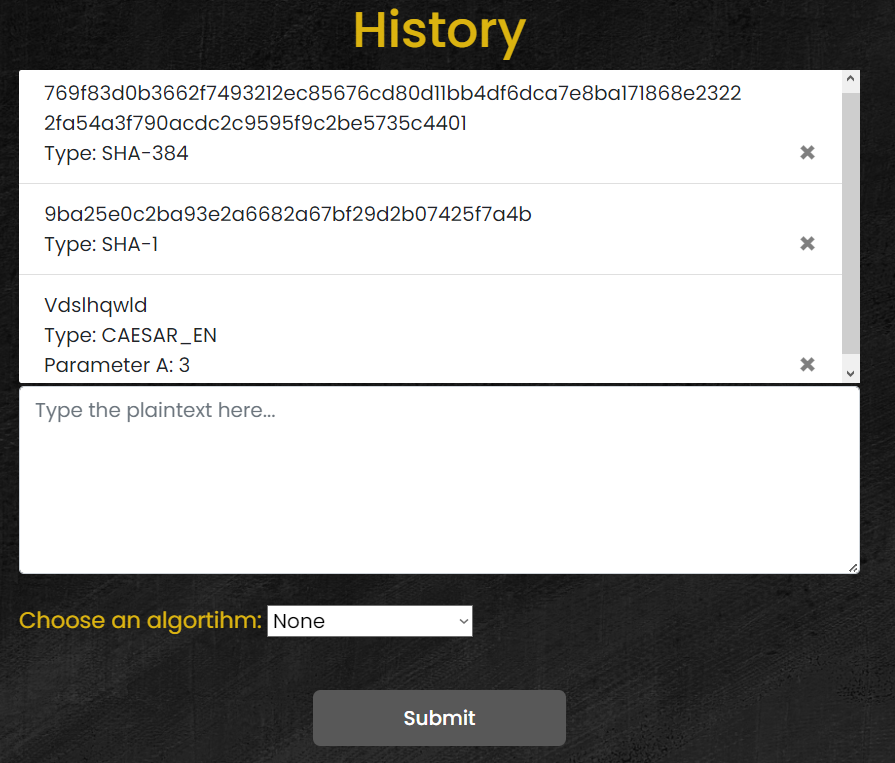
\includegraphics[scale=0.45]{images/cryptBase}
	\caption{Crypt felület}
	\label{fig:cryptBase}
\end{figure}

	%----------------------------------------------------------------------------
\chapter{Továbbfejlesztési lehetőségek}
%----------------------------------------------------------------------------


\textbf{Bővített kriptográfiai rendszerek:} Az alkalmazásba további kriptográfiai rendszerek, mint például Salsa20, ElGamal vagy ECC (Elliptic Curve Cryptography) integrálása lehetőséget adna a felhasználóknak a különböző algoritmusok kipróbálására és tanulására. Továbbá megfontolandó lenne az AES titkosító további módjainak beépítésére.

\textbf{Interaktív gyakorló feladatok:} Interaktív gyakorló feladatok készítése, amelyek segítségével a felhasználók a tanulói felületen gyakorolhatják a különböző kriptográfiai rendszerek alkalmazását. Ez javítaná a gyakorlati tapasztalatok szerzését és a tanulás hatékonyságát.

\textbf{Felhasználói profilok és eredmények nyomon követése:} Egy felhasználói profil rendszer létrehozása, ahol a felhasználók módosíthatják adataikat és nyomon követhetik a teljesítményt, például az elért eredményeket vagy az elvégzett feladatokat. Ez segít a felhasználóknak a fejlődésük nyomon követésében és motivációjuk fokozásában.

\textbf{További nyelvi támogatás:} Az alkalmazást további nyelvek támogatásával való kibővítése, hogy a nem angol vagy magyar anyanyelvű felhasználók is könnyen használhassák és megértsék a rendszert. Ez növelné a felhasználói kört és a felhasználói elégedettséget.

\textbf{Reszponzív dizájn:} Az alkalmazás biztosítása a különböző eszközökön történő használathoz.

\vspace{10pt}
Ezek a továbbfejlesztési lehetőségek hozzájárulhatnak az alkalmazás funkcionalitásának és felhasználói élményének javításához, valamint a felhasználók kriptográfiai ismereteinek bővítéséhez.
	%----------------------------------------------------------------------------
\chapter*{Összefoglaló}\addcontentsline{toc}{chapter}{Összefoglaló}
%----------------------------------------------------------------------------

A Cryptorithm egy webes alkalmazás, amely lehetővé teszi a felhasználók számára különböző kriptográfiai rendszerek kipróbálását és tanulását. Az alkalmazásban számos beépített kriptográfiai eszköz áll rendelkezésre, mint például az SHA, Whirlpool és bcrypt hashelés, a Blowfish, ChaCha20 titkosítók, az AES titkosítás CTR módban, valamint az Affin és Caesar rejtjelezések. A felhasználók a felületen keresztül kiválaszthatják, hogy melyik rendszert szeretnék alkalmazni, és gyakorolhatnak a megértéséhez. Az alkalmazás intuitív felhasználói felülettel rendelkezik és támogatja a többnyelvűséget. A Cryptorithm célja, hogy segítse a felhasználókat a kriptográfiai ismeretek bővítésében, miközben egy interaktív és tanulást támogató környezetet biztosít.

GitHub link: \url{https://github.com/zali07/Cryptorithm}

% Koszonetnyilvanitas
%~~~~~~~~~~~~~~~~~~~~~~~~~~~~~~~~~~~~~~~~~~~~~~~~~~~~~~~~~~~~~~~~~~~~~~~~~~~~~~~~~~~~~~
	%----------------------------------------------------------------------------
\chapter*{\koszonetnyilvanitas}\addcontentsline{toc}{chapter}{\koszonetnyilvanitas}
%----------------------------------------------------------------------------

Szeretném kifejezni hálámat a családomnak és barátaimnak, akik támogattak és bátorítotak engem ezen az úton. Köszönet illeti a vezető tanáromat is, aki értékes útmutatást és iránymutatást nyújtott a projekt fejlesztése során.


% Tablazatok es abrak jegyzeke (EZ NEM KOTELEZO)
%~~~~~~~~~~~~~~~~~~~~~~~~~~~~~~~~~~~~~~~~~~~~~~~~~~~~~~~~~~~~~~~~~~~~~~~~~~~~~~~~~~~~~~
	\listoffigures\addcontentsline{toc}{chapter}{\abrakjegyzeke}
%	\listoftables\addcontentsline{toc}{chapter}{\tablazatokjegyzeke}


% Bibliography
%~~~~~~~~~~~~~~~~~~~~~~~~~~~~~~~~~~~~~~~~~~~~~~~~~~~~~~~~~~~~~~~~~~~~~~~~~~~~~~~~~~~~~~
	\bibliography{mybib}
	\addcontentsline{toc}{chapter}{\irodalomjegyzek}
	\bibliographystyle{alpha}
	
% Appendix
%~~~~~~~~~~~~~~~~~~~~~~~~~~~~~~~~~~~~~~~~~~~~~~~~~~~~~~~~~~~~~~~~~~~~~~~~~~~~~~~~~~~~~~
%	%----------------------------------------------------------------------------
\appendix
%----------------------------------------------------------------------------
\chapter*{\fuggelek}\addcontentsline{toc}{chapter}{\fuggelek}
\setcounter{chapter}{6}  % a fofejezet-szamlalo az angol ABC 6. betuje (F) lesz
\setcounter{equation}{0} % a fofejezet-szamlalo az angol ABC 6. betuje (F) lesz
\numberwithin{equation}{section}
\numberwithin{figure}{section}
\numberwithin{lstlisting}{section}
%\numberwithin{tabular}{section}

%----------------------------------------------------------------------------
\section{A TeXworks felülete}
%----------------------------------------------------------------------------
\begin{figure}[!ht]
\centering
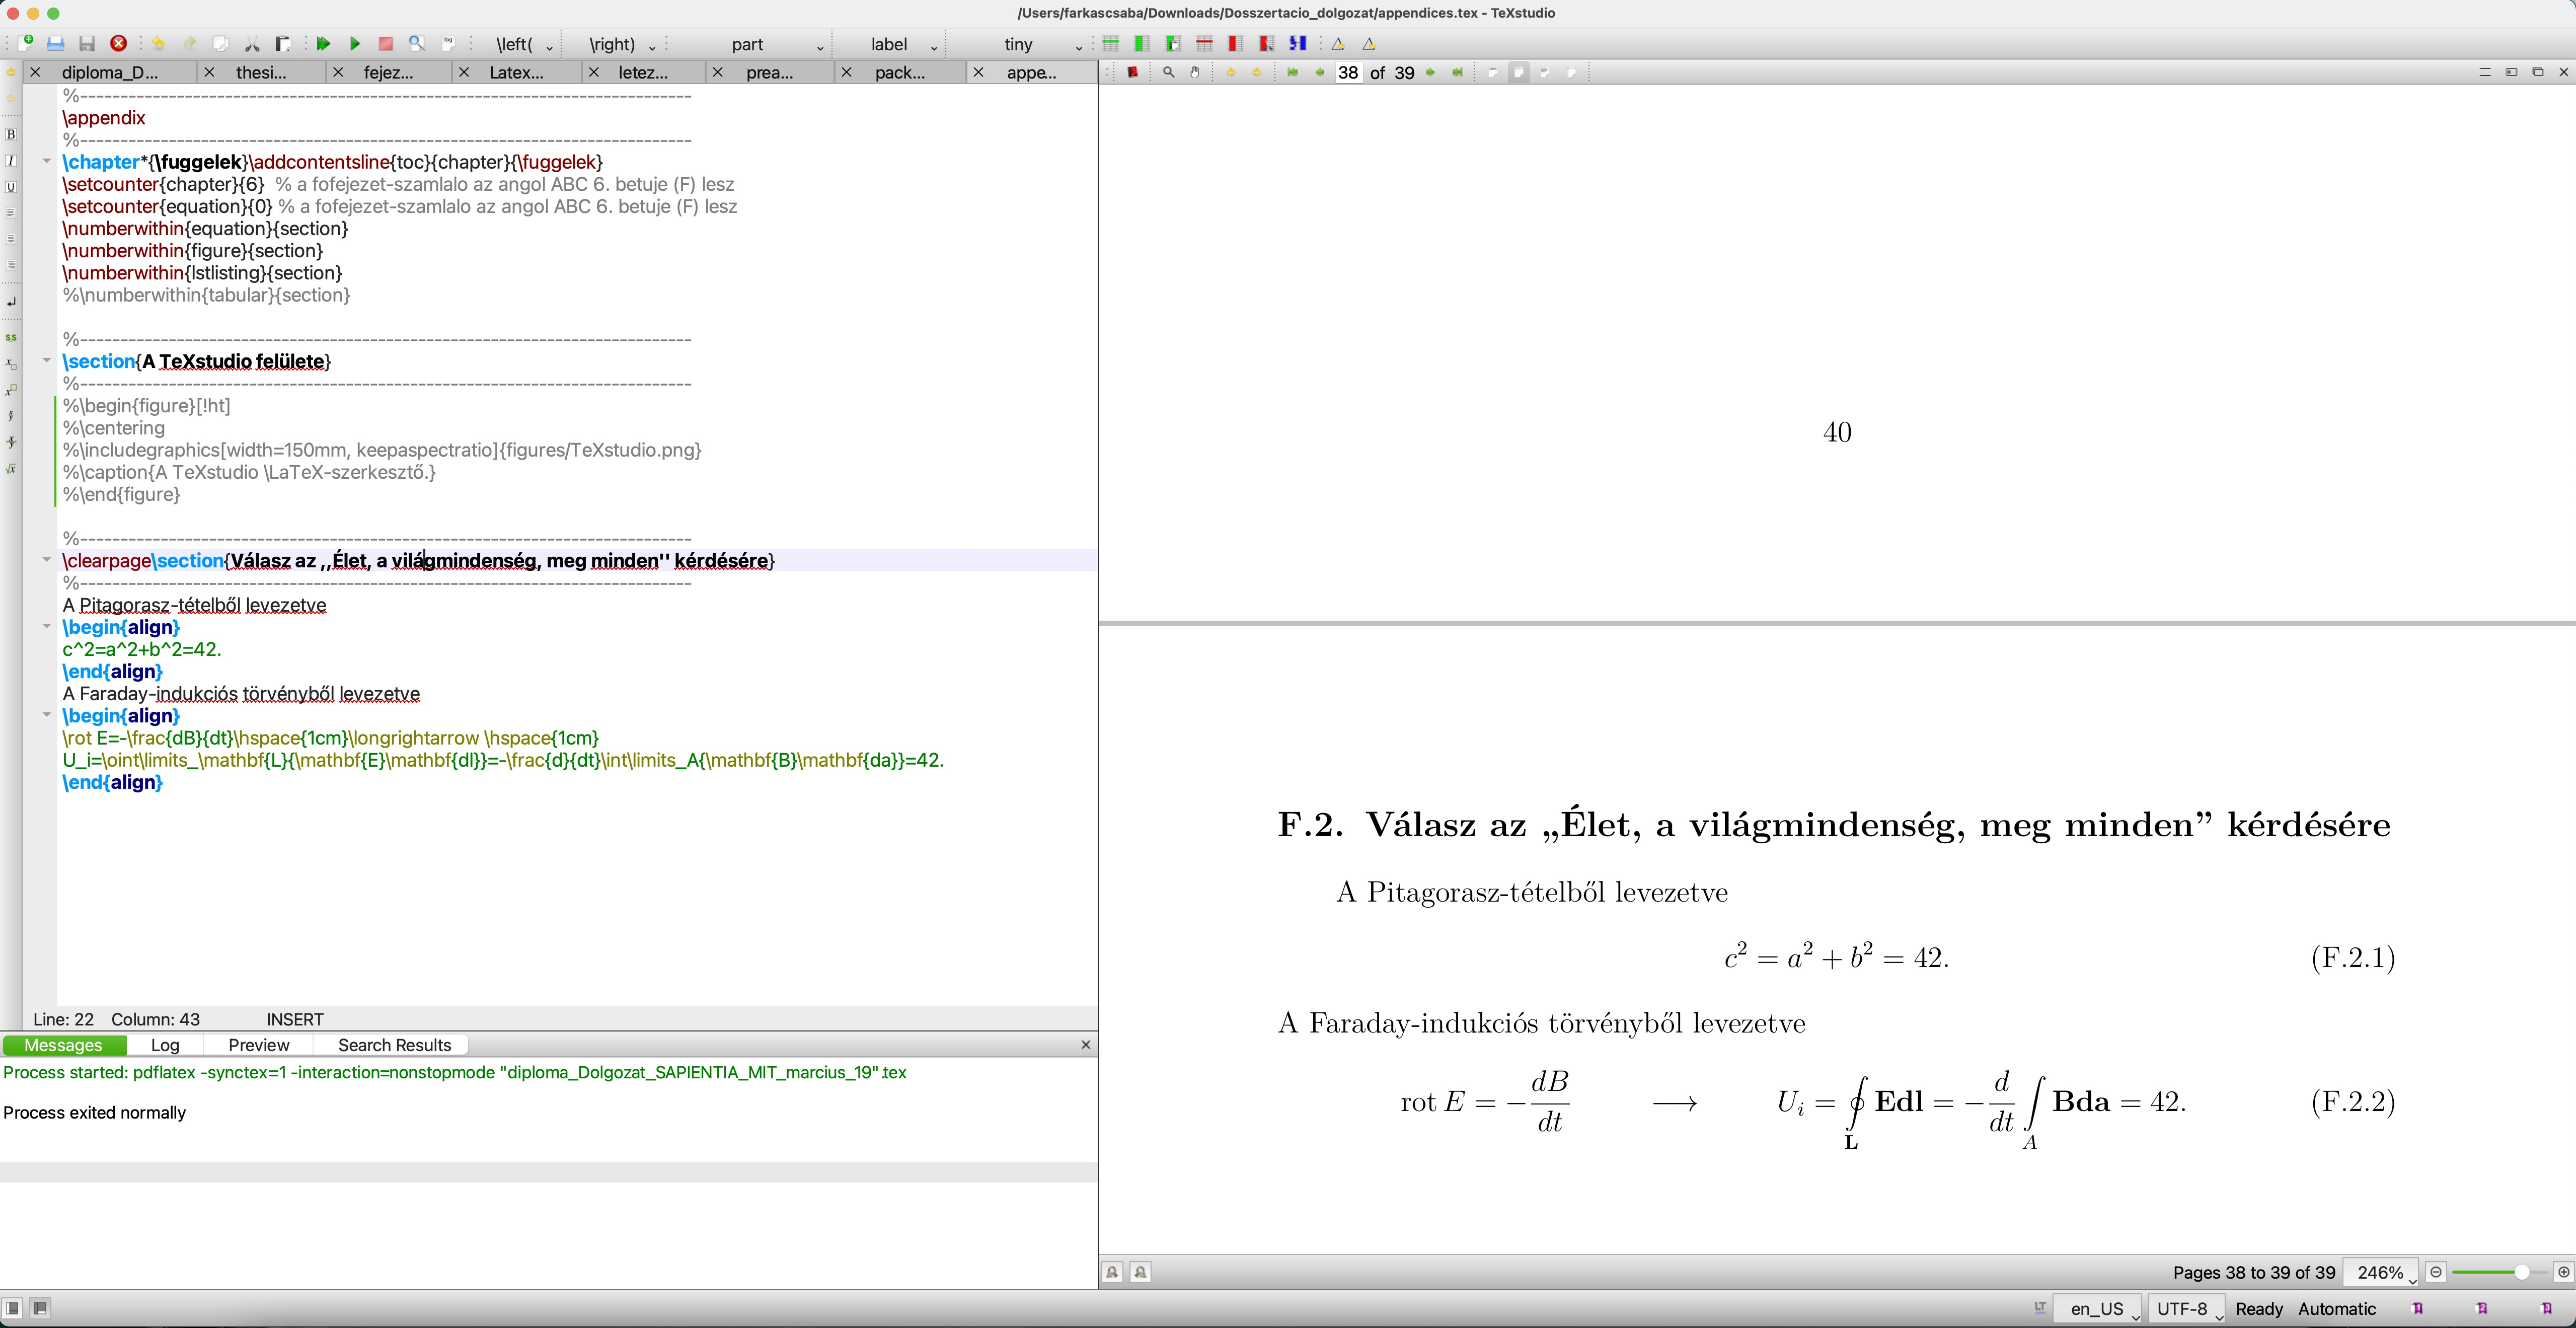
\includegraphics[width=150mm, keepaspectratio]{images/texstudio}
\caption{A TeXworks \LaTeX-szerkesztő.} 
\end{figure}







\label{page:last}
\end{document}
